\section{Nonlinear Latent Variable Models}

  Now we will consider ourselves with nonlinear latent variables models, which still defines a simple latent random variable $Z$ with prior $p(z)$, but now a family of nonlinear functions $\{f_\theta (z)\}$ that defines the generative component $f_\theta (x \mid z)$. In factor models, we have taken linear transformations of random variables and therefore the likelihood had been easy to calculate, differentiate, and therefore optimize. 

  In the general nonlinear case, we usually deal with $f_\theta$ not as a transformation of $Z$ to $X$, but really $f_\theta (z)$ becomes the \textit{parameters} of $X \mid Z = z$. This allows to define the \textit{implicitly parameterized} family of distributions $\{p_\theta\}$. Given that the true distribution of the data is $p^\ast (x)$, we would like to find a distribution $p_\theta (x)$ that is a good approximation. 
  \begin{equation}
    p^\ast (x) \approx p_\theta (x)
  \end{equation}
  To calculate the likelihood $p_\theta (x)$, we must compute the marginal 
  \begin{equation}
    p_\theta (x) = \int p_\theta (x, z) \,dz = \int p_\theta (x \mid z) \, p(z) \,dz
  \end{equation}
  which is known to be computationally intractable due to the integral. At first, it seems like all hope is lost, but statisticians have a few tricks up their sleeves. 
  \begin{enumerate} 
    \item The first trick is to notice that by Bayes rule, we can compute the likelihood not as an integral, but as 
    \begin{equation}
      p_\theta (x) = \frac{p_\theta (x \mid z) \, p(z)}{p_\theta (z \mid x)} 
    \end{equation}
    So it suffices to find a good approximation of $p_\theta (z \mid x)$, which is a probabilistic discriminative model for the latent variable (i.e. we are trying to compute the distribution of $z$ given $x$ as if we were predicting it). We can do MCMC since $p_\theta (z \mid x) \propto p_\theta (x \mid z) \, p(z)$, but often this can be slow to fit. 

    \item The next trick is called the variational lower bound, which is a lower bound on the log likelihood, and therefore by optimizing it we can hope to optimize the log-likelihood as well. This works well in practice. 

    \item The next trick is by optimizing the Fisher score, which is the gradient of the log likelihood \textit{with respect to the covariates} (not the parameters!). 
  \end{enumerate}

\subsection{Variational Lower Bounds} 

  We focus on this problem and define a family of distributions $\{q_\phi (z \mid x)\}_\phi$ and use it to approximate $p_\theta (z \mid x)$. Therefore, searching for a good $\phi$ and therefore a good $q_\phi$ is basically the problem of \textbf{variational Bayesian inference}. Essentially we are trying to construct an encoder and a decoder.

  \begin{figure}[H]
    \centering 
    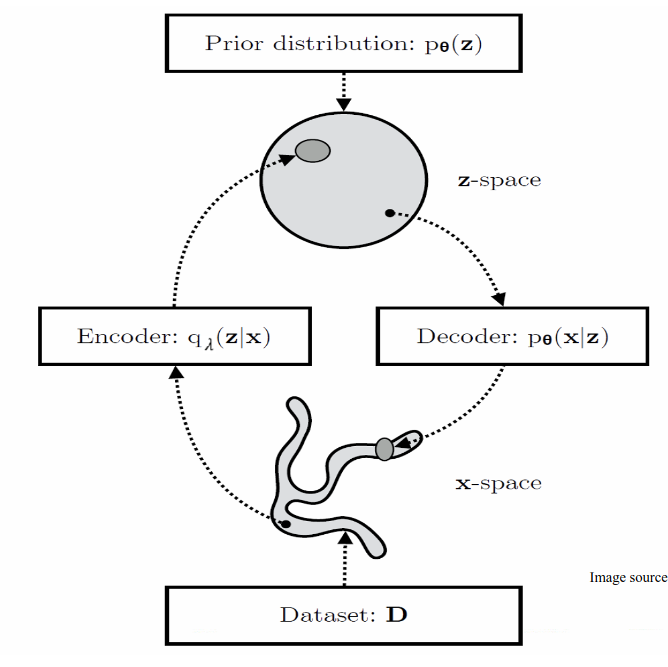
\includegraphics[scale=0.4]{img/VAE_framework.png}
    \caption{If $q_{\phi} = p_{\theta}$, then the diagram commutes, i.e. $p(z) p_{\theta}(x \mid z) = p(x) p_{\theta}(z \mid x) = p_{\theta} (x, z)$.} 
    \label{fig:vae_framework}
  \end{figure}

  As we have stated before (and in pretty much all density estimation problems), our job is to maximize the log likelihood of the training set: 
  \begin{equation}
    \sum_{i} \log p(x^{(i)})
  \end{equation}

  In order to do this for this problem, we need a little fact from information theory. 

  \begin{theorem}[Log Likelihood vs Conditional Entropy]
    The KL divergence can be decomposed to 
    \begin{equation}
      KL \big( q_\phi (z \mid x) \mid\mid p_{\theta} (z \mid x) \big) = \mathbb{E}_{q_\phi(z \mid x)} [ \log q_{\phi} (z \mid x)] + \log p_{\theta} (x) - \mathbb{E}_{q_{\phi} (z \mid x)} [\log p_{\theta} (x, z)]
    \end{equation}
    and hence 
  \end{theorem}
  \begin{proof}
    Starting with the definition of KL divergence:
    \begin{align}
      KL(q_\phi(z \mid x) \mid\mid p_\theta(z \mid x)) &= \mathbb{E}_{q_\phi(z \mid x)}\left[\log \frac{q_\phi(z \mid x)}{p_\theta(z \mid x)}\right] \\
      &= \mathbb{E}_{q_\phi(z \mid x)}[\log q_\phi(z \mid x)] - \mathbb{E}_{q_\phi(z \mid x)}[\log p_\theta(z \mid x)]
    \end{align}

    By Bayes' rule, we know that
    \begin{equation}
      p_\theta(z \mid x) = \frac{p_\theta(x, z)}{p_\theta(x)}
    \end{equation}

    Substituting this into our equation gives 
    \begin{align}
      KL(q_\phi(z \mid x) \mid\mid p_\theta(z \mid x)) &= \mathbb{E}_{q_\phi(z \mid x)}[\log q_\phi(z \mid x)] - \mathbb{E}_{q_\phi(z \mid x)}\left[\log \frac{p_\theta(x, z)}{p_\theta(x)}\right] \\
      &= \mathbb{E}_{q_\phi(z \mid x)}[\log q_\phi(z \mid x)] - \mathbb{E}_{q_\phi(z \mid x)}[\log p_\theta(x, z)] + \mathbb{E}_{q_\phi(z \mid x)}[\log p_\theta(x)]
    \end{align}

    Since $\log p_\theta(x)$ is constant with respect to $z$, we can take it out of the expectation. 
    \begin{equation}
      \mathbb{E}_{q_\phi(z \mid x)}[\log q_\phi(z \mid x)] - \mathbb{E}_{q_\phi(z \mid x)}[\log p_\theta(x, z)] + \log p_\theta(x)
    \end{equation}
  \end{proof}

  Therefore maximizing the log-likelihood is equivalent to minimizing the KL-divergence. 
  \begin{equation}
    \log p_\theta (x) = KL \big( q_\phi (z \mid x) \mid\mid p_{\theta} (z \mid x) \big) + \mathbb{E}_{q_{\phi} (z \mid x)} [\log p_{\theta} (x, z)] - \mathbb{E}_{q_\phi(z \mid x)} [ \log q_{\phi} (z \mid x)]
  \end{equation}
  But again the KL divergence part is intractable due to $p_\theta (z \mid x)$ being intractable. Using the fact that the KL divergence is always greater than or equal to $0$, we can drop the term and set a lower bound on the log likelihoods. This lower bound is called the \textit{variational lower bound}.  
  \begin{equation}
    \sum_{i=1}^N \log p_{\theta} (x^{(i)}) \geq \sum_{i=1}^N \mathbb{E}_{q_\phi (z \mid x^{(i)})} [ \log p_{\theta} (x^{(i)}, z)] - \sum_{i=1}^N \mathbb{E}_{q_{\phi} (z \mid x^{(i)})} [ \log q_{\phi} (z \mid x^{(i)}) ]
  \end{equation} 

  \begin{definition}[Variational Lower Bound]
    The \textbf{variational lower bound} of the dataset $\mathcal{D}$ is defined 
    \begin{equation}
      \elbo(\mathcal{D}, \phi, \theta) = \sum_{i=1}^N \mathbb{E}_{q_\phi (z \mid x^{(i)})} [ \log p_{\theta} (x^{(i)}, z)] - \sum_{i=1}^N \mathbb{E}_{q_{\phi} (z \mid x^{(i)})} [ \log q_{\phi} (z \mid x^{(i)})] 
    \end{equation}
    which can be decomposed into the sums of the variational lower bounds of the individual data points. 
    \begin{equation}
      \elbo(\mathcal{D}, \phi, \theta) = \elbo(x^{(i)}, \phi, \theta) 
    \end{equation}
    where 
    \begin{equation}
      \elbo(x^{(i)}, \phi, \theta) = \mathbb{E}_{q_\phi (z \mid x^{(i)})} [ \log p_{\theta} (x^{(i)}, z)] - \mathbb{E}_{q_{\phi} (z \mid x^{(i)})} [ \log q_{\phi} (z \mid x^{(i)})] 
    \end{equation}
  \end{definition}

  Note that we can alternatively define ELBO using Jensen's inequality. 

  \begin{definition}[Evidence Lower Bound]
    To lower bound it, we can use Jensen's inequality\footnote{Given convex function $f: \mathbb{R} \rightarrow \mathbb{R}$, and random variable $X$, $\mathbb{E}[f(x)] \geq f(\mathbb{E}[X])$.} with the concave function $f(x) = \log(x)$ over domain $\mathbb{R}^+$ and the following holds true for all $\theta$ and more importantly, for \textit{any arbitrary density function} $q(z)$. Therefore, we have 
    \begin{align}
      \ell(\theta) & = \log p_\theta (x) \\
                   & = \log \int p_\theta (x, z) \,dz \\
                   & = \log \int q_\phi (z) \frac{p_\theta (x, z)}{q_\phi (z)} \,dz \\ 
                   & \geq \int q_\phi (z \mid x) \log \bigg( \frac{p_\theta (x, z)}{q_\phi (z)} \bigg) \,dz \\  
                   & = \elbo(x, q_\phi)
    \end{align}
    The lower bound is called the \textbf{evidence lower bound (ELBO)}, and the ELBO of the whole dataset is 
    \begin{equation}
      \elbo(\mathcal{D}, \phi, \theta) = \sum_{i=1}^N \elbo(x^{(i)}, \phi, \theta)
    \end{equation}
  \end{definition} 

  Note that this lower bound is with respect to \textit{any} distribution $q_\phi$, and it is because of this flexibility that we choose $q_\phi$ in the first place. Therefore, we can vary $\phi$ in hopes that the lower bound is maximized, and optimize with respect to this, hence the name \textit{variational}. For more interpretability, look at the corollary. 

  \begin{corollary}[Decomposition of ELBO]
    The following decomposition of ELBO shows that maximizing the ELBO simultaneously attempts to keep $q_\phi$ close to $p$ and concentrate $q_\phi(z \mid x)$ on those $z$ that maximizes $\ln p_\theta (x \mid z)$. That is, the approximate posterior $q_\phi$ balances between staying close to the prior $p(z)$ and moving towards the maximum likelihood $\argmax_z \ln p_\theta (x \mid z)$. 
    \begin{equation}
      \elbo(x^{(i)}, \phi, \theta) = \underbrace{\mathbb{E}_{q_\phi (z \mid x^{(i)})} [\log p_{\theta} (x^{(i)} \mid z)]}_{\substack{\text{likelihood term} \\ \text{(reconstruction part)}}}- \underbrace{KL(q_{\phi} (z \mid x^{(i)}) \mid\mid p(z))}_{\substack{\text{closeness of encoding to } p(z) \\ \text{(typically Gaussian)}}}
    \end{equation}
    Note the first expression is the likelihood term, which measures the reconstruction quality of the decoder $p_\theta(x^{(i)} \mid z)$ averaged over encodings sampled from $q_\phi(z \mid x^{(i)})$. The second term is the KL divergence between the encoder distribution $q_\phi(z \mid x^{(i)})$ and the prior $p(z)$, which acts as a regularizer by ensuring the encoded distributions remain close to the chosen prior, typically a standard normal distribution.
  \end{corollary}
  \begin{proof}
    Starting with the ELBO for a single data point:
    \begin{align*}
      \elbo(x^{(i)}, \phi, \theta) &= \mathbb{E}_{q_\phi(z \mid x^{(i)})}[\log p_\theta(x^{(i)}, z)] - \mathbb{E}_{q_\phi(z \mid x^{(i)})}[\log q_\phi(z \mid x^{(i)})]
    \end{align*}

    Using the chain rule of probability for the joint distribution:
    \begin{align*}
      p_\theta(x^{(i)}, z) = p_\theta(x^{(i)} \mid z)p(z)
    \end{align*}

    Substituting this into our ELBO:
    \begin{align*}
      \elbo(x^{(i)}, \phi, \theta) &= \mathbb{E}_{q_\phi(z \mid x^{(i)})}[\log p_\theta(x^{(i)} \mid z) + \log p(z)] - \mathbb{E}_{q_\phi(z \mid x^{(i)})}[\log q_\phi(z \mid x^{(i)})] \\
      &= \mathbb{E}_{q_\phi(z \mid x^{(i)})}[\log p_\theta(x^{(i)} \mid z)] + \mathbb{E}_{q_\phi(z \mid x^{(i)})}[\log p(z)] - \mathbb{E}_{q_\phi(z \mid x^{(i)})}[\log q_\phi(z \mid x^{(i)})] \\
      &= \mathbb{E}_{q_\phi(z \mid x^{(i)})}[\log p_\theta(x^{(i)} \mid z)] - \left(\mathbb{E}_{q_\phi(z \mid x^{(i)})}[\log q_\phi(z \mid x^{(i)})] - \mathbb{E}_{q_\phi(z \mid x^{(i)})}[\log p(z)]\right) \\
      &= \underbrace{\mathbb{E}_{q_\phi(z \mid x^{(i)})}[\log p_\theta(x^{(i)} \mid z)]}_{\text{reconstruction term}} - \underbrace{KL(q_\phi(z \mid x^{(i)}) \mid\mid p(z))}_{\text{KL divergence term}}
    \end{align*}
  \end{proof} 

  The next step is to actually maximize the ELBO with respect to both $\theta$ and $\phi$. To do this we need to compute the derivatives of $\elbo$ w.r.t. to $\phi$ and $\theta$. 

  \begin{equation}
    \max_{\phi, \theta} \elbo(\mathcal{D}, \phi, \theta)
  \end{equation}
  It turns out that this itself is a nonconvex optimization problem, and to make it doable we iterate between updating $\phi$ and $\theta$. 

  \begin{lemma}[Gradient of ELBO w.r.t. $\theta$]
    For $\theta$, we can obtain its unbiased gradient as such
    \begin{align} 
      \nabla_\theta \elbo(x, \theta, \phi) & = \nabla_\theta \big\{ \mathbb{E}_{q_\phi (z \mid x)} [ \log p_\theta (x, z)] - \mathbb{E}_{q_\phi (z \mid x)} [\log q_{\phi} (z \mid x)] \} \\
                                           & = \mathbb{E}_{q_\phi (z \mid x)} \big[ \nabla_\theta \{ \log p_\theta (x, z) - \log q_{\phi} (z \mid x) \}  \big] \\
                                           & \approx \nabla_\theta \big\{ \log p_\theta(x, z) - \log q_\theta (z \mid x) \big\} \\
                                           & = \nabla_\theta \log p_\theta (x, z) 
    \end{align}
    where the step with the $\approx$ just indicates that we approximate the expectation with a sample of size $1$ over some minibatch. 
  \end{lemma}

  However, taking the gradient w.r.t. $\phi$ is more complicated since we cannot put the gradient in the expectation, i.e. swap the derivative and integral (since we are deriving and integrating w.r.t. $\phi$). 

  \begin{lemma}[Gradient of ELBO w.r.t. $\phi$ with Score Function Estimators]
    To handle the gradient with respect to $\phi$, we can use the score function estimator (also known as REINFORCE):

    \begin{align}
      \nabla_\phi \elbo(x, \theta, \phi) &= \nabla_\phi \mathbb{E}_{q_\phi(z|x)}[\log p_\theta(x,z) - \log q_\phi(z|x)] \\
      &= \mathbb{E}_{q_\phi(z|x)}[\nabla_\phi \log q_\phi(z|x)(\log p_\theta(x,z) - \log q_\phi(z|x))]
    \end{align}

    This identity follows from the log-derivative trick:
    \begin{equation}
      \nabla_\phi \mathbb{E}_{q_\phi(z)}[f(z)] = \mathbb{E}_{q_\phi(z)}[f(z)\nabla_\phi \log q_\phi(z)]
    \end{equation}
  \end{lemma}

  Now that we have approximate closed form solutions for the gradients, we can optimize the two using coordinate ascent. 

  \begin{algo}[Coordinate Ascent Variational Inference]
    A common approach to maximize the ELBO is coordinate ascent, where we alternatively optimize with respect to $q_\phi$ and $\theta$:

    \begin{algorithm}[H]
      \caption{Coordinate Ascent Variational Inference (CAVI)}
      \begin{algorithmic}[1]
        \Require Initial parameters $\theta^{(0)}$, $\phi^{(0)}$
        \While{not converged}
          \State // E-step: optimize variational parameters
          \State $\phi^{(t+1)} \gets \argmax_\phi \elbo(\mathcal{D}, \phi, \theta^{(t)})$
          \State // M-step: optimize model parameters
          \State $\theta^{(t+1)} \gets \argmax_\theta \elbo(\mathcal{D}, \phi^{(t+1)}, \theta)$
        \EndWhile
      \end{algorithmic}
    \end{algorithm}
  \end{algo}
  
\subsection{EM Algorithm}

  The coordinate ascent approach reveals the deep connection between variational inference and the EM algorithm. In fact, the EM algorithm can be viewed as a special case where:

  \begin{itemize}
    \item The E-step finds the exact posterior $q_\phi(z|x) = p_\theta(z|x)$ rather than approximating it
    \item The M-step maximizes the expected complete data log-likelihood
  \end{itemize}

  When the exact posterior is intractable, variational inference provides an approximate alternative to EM by:
  \begin{equation}
    q_\phi(z|x) \approx p_\theta(z|x)
  \end{equation}

  This leads to the variational EM algorithm:

  \begin{enumerate}
    \item Variational E-step: Find $q_\phi$ that best approximates the posterior
    \begin{equation}
      \phi^{(t+1)} = \argmin_\phi KL(q_\phi(z|x) || p_{\theta^{(t)}}(z|x))
    \end{equation}
    
    \item M-step: Maximize the expected complete data log-likelihood under $q_\phi$
    \begin{equation}
      \theta^{(t+1)} = \argmax_\theta \mathbb{E}_{q_{\phi^{(t+1)}}(z|x)}[\log p_\theta(x,z)]
    \end{equation}
  \end{enumerate}

  This framework provides a systematic way to perform approximate inference when exact EM is intractable.

\subsection{Bruh}

  Suppose we have an estimation problem given the training set $\{x^{(i)}\}_{i=1}^n$. We have latent variable model $p(x, z; \theta)$ with $z$ being the latent variable of discrete, finite random variable $Z$, with density $p_Z (z)$. Let us denote the density of $X$ as $p_X$. Then, the random variable $X$ can be interpreted as us first generating $z$ from $Z$, and then computing $X\,|\,Z = z$.  
  \[\text{Compute } X = \text{Compute } Z \text{ and then } \begin{cases} 
  \text{Compute } X \,|\, Z = 1 \\
  \text{Compute } X \,|\, Z = 2 \\
  \ldots \\
  \text{Compute } X \,|\, Z = k
  \end{cases}\]

  Let us clarify some notation: 
  \begin{itemize}
    \item The distribution that we will iteratively reassign over and over again is $Z$, with density $p_Z$ that maps $z \mapsto \phi_z$, where $\phi$ is a vector that represents the density.
    \item The $k$ conditional (not necessarily Gaussian) distributions that we will iteratively reassign over and over again is $X_1, X_2, \ldots, X_k$, with densities $p_{X_1} (x), \ldots, p_{X_k} (x)$ that maps $x \mapsto p_{X_j} (x)$.
    \item The distribution of the entire random variable $X$ will have density $p_X (x)$. Since we are iteratively reassigning the densities $p_Z$ and $p_{X_j}$, this joint distribution of $X$ will also get modified.
  \end{itemize}

  The EM algorithm in the general case has the following steps: 
  \begin{enumerate}
    \item We initialize the value of $\theta$ in some way. Note that within this $\theta$ are the parametizations of the initial multinomial density $p_Z$, which is our initial "guess" of the distribution of $Z$.
    \item \textbf{(E Step)} The log likelihood of the given data $\{ x^{(i)}\}_{i=1}^n$ with respect to the parameter $\theta$ (which encodes all parameters of distribution $Z$ and all $X\,|\,Z$) is 
      \[l(\theta) = \sum_{i=1}^n \log\, p_X \big( x^{(i)}; \, \theta \big)\]
    It turns out that explicitly finding the maximum likelihood estimates of the parameters $\theta$ is hard because it results in a difficult, non-convex optimization problem. So, we tackle this another way. 
    
    To start, we can see that the summation isn't too crucial, so we can focus on minimizing each $\log \, p_X \big(x^{(i)}; \, \theta \big)$ and summing in the end. We can calculate this by conditioning over all $j = 1, \ldots, k$ generated from $Z$ (which we have guessed to have an initial density of $p_Z$). That is, we must find for each $i = 1, 2, \ldots, n$ 
    \begin{align*} 
      \max_\theta \log \, p_X \big( x^{(i)}; \, \theta \big) & = \max_\theta \log \, \bigg(\sum_{j=1}^k p_X \big(x^{(i)}, Z = j; \, \theta\big) \bigg) \\
      & = \max_\theta \log \bigg( \sum_{j=1}^k p_X \big( x^{(i)}\,|\, Z = j; \, \theta\big) p_Z \big( j; \, \theta \big) \bigg) \\
      & = \max_\theta \log \bigg( \sum_{j=1}^k p_{X_j} \big( x^{(i)} ;\, \theta\big) p_Z \big( j; \, \theta \big) \bigg)
    \end{align*}
    To find this maximum value, we can focus on the first equality and see that by Jensen's inequality (with conCAVE, not convex, $f(x) = \log x$ over domain $x \in \mathbb{R}^+$), the following holds true for all $\theta$ and more importantly, for \textit{any arbitrary density function} $p_Z^{*i}$.  
    \begin{align*} 
      \log p_X \big(x^{(i)};\, \theta\big) & = \log \bigg( \sum_{j=1}^k p_X \big(x^{(i)}, Z = j;\, \theta \big) \bigg) \\ 
      & = \log \bigg( \sum_{j=1}^k p_Z^{*i} \big(j \big)\, \frac{p_X \big(x^{(i)}, Z = j;\, \theta \big)}{p_Z^{*i} \big(j \big)} \bigg) \\
      & = \log \Bigg(\mathbb{E}_{j \sim p_Z^{*i}} \bigg( \frac{p(x^{(i)}, Z = j; \, \theta)}{p_Z^{*i} \big(j \big)}\bigg)\Bigg) \\
      & \geq \mathbb{E}_{j \sim p_Z^{*i}} \Bigg( \log \bigg( \frac{p(x^{(i)}, Z = j; \, \theta)}{p_Z^{*i} \big(j \big)} \bigg) \Bigg) \\
      & = \sum_{j=1}^k p_Z^{*i} (j) \, \log\bigg( \frac{p(x^{(i)}, Z = j; \, \theta)}{p_Z^{*i} (j)} \bigg) = \text{ELBO} \big( x^{(i)}; \,p_Z^{*i}, \theta \big)
    \end{align*}
    The final term, called the \textbf{evidence lower bound} (ELBO), is just the expectation of $\log \frac{p(x^{(i)}, Z = j; \, \theta)}{p_Z^{*i} (j)}$ with respect to $j$ drawn from density $p_Z^{*i}$, which is denoted with $\mathbb{E}_{j \sim p_Z^{*i}}$. 
    
    Summing over all $n$ examples, we have a lower bound for the entire log likelihood for \textit{any} set of density functions $p_Z^{*1}, p_Z^{*2}, \ldots, p_Z^{*n}$: 
    \begin{align*} 
      l(\theta) = \sum_{i=1}^n \log p(x^{(i)}; \, \theta) & \geq \sum_{i=1}^n \text{ELBO}(x^{(i)}; \, p_Z^{*i}, \theta) \\
      & = \sum_{i=1}^n \sum_{j=1}^k p_Z^{*i} (j) \, \log\bigg( \frac{p(x^{(i)}, Z = j; \, \theta)}{p_Z^{*i} (j)} \bigg)
    \end{align*}
    Our job now is to choose the correct density functions $p_Z^{*i}$'s such that the lower bound is maximized. It turns out that we can do even better: equality is satisfied if and only if we set 
    \begin{align*} 
      p_Z^{*i} (j) & \equiv p_Z \big( j\,|\, x^{(i)}; \, \theta \big) \\
      & \equiv p_Z^{(i)} \big( j; \, \theta \big) \text{ for all } i = 1, 2, \ldots, n
    \end{align*}
    which is simply the posterior distribution of the multinomial given the observed sample $x^{(i)}$, which we can easily calculate using Bayes' rule. Substituting this into $p_Z^{*i}$ leads to the equality 
    \begin{align*} 
      l(\theta) = \sum_{i=1}^n \log p (x^{(i)}; \, \theta) 
      & = \sum_{i=1}^n \text{ELBO}\big(x^{(i)}; p_Z^{(i)}, \, \theta \big) \\
      & = \sum_{i=1}^n \sum_{j=1}^k p_Z^{(i)} \big( j; \, \theta \big) \, \log\bigg( \frac{p(x^{(i)}, Z = j; \, \theta)}{p_Z^{(i)} \big( j; \, \theta \big)} \bigg) \\
      & = \sum_{i=1}^n \sum_{j=1}^k p_Z \big( j\,|\, x^{(i)}; \, \theta \big) \, \log\bigg( \frac{p(x^{(i)}, Z = j; \, \theta)}{p_Z \big( j\,|\, x^{(i)}; \, \theta \big)} \bigg)
    \end{align*}
    In summary, this E step has taken the log-likelihood function $l(\theta)$ (representing (the log of) the probability of all the $x^{(i)}$'s landing where they are given the parameters $\theta$), which is abstract and hard-to-optimize, and converted it into an equivalent form as the sum of a bunch of ELBO functions optimized with the density parameters begin assigned $p_Z^{*i} = p_Z^{(i)}$. 
    
    But remember that these optimal densities $p_Z^{*i} = p_Z^{(i)}$ make the right and left hand side equivalent only for a \textbf{fixed value} of $\theta$! So, the right hand side is only equivalent to $l(\theta)$ only for that one value of $\theta$, but as soon as we set $\theta$ to something else, the right hand side evaluated with $p_Z^{*i} = p_Z^{(i)}$ are not equal.
    \item \textbf{(M Step)} Since we have found some equivalent form of $l(\theta)$ for the fixed $\theta$ that was initialized, we can now just maximize the right hand side with respect to $\theta$, while fixing the $p_Z^{*i} = p_Z^{(i)}$'s. Therefore, we find and set the value of $\theta$ as 
    \begin{align*}  
      \theta & = \text{arg}\; \max_\theta \sum_{i=1}^n \text{ELBO} \big( x^{(i)}; \, p_Z^{(i)}, \theta \big) \\
      & = \text{arg}\; \max_\theta \sum_{i=1}^n \sum_{j=1}^k p_Z^{(i)} (j)\; \log \bigg( \frac{p(x^{(i)}, Z = j; \, \theta)}{p_Z^{(i)} (j)} \bigg) \\
      & = \text{arg}\; \max_\theta \sum_{i=1}^n \sum_{j = 1}^k p_Z \big(j\,|\, x^{(i)}; \, \theta \big)\, \log \bigg( \frac{p(x^{(i)}, Z = j; \, \theta)}{p_Z \big(j\,|\, x^{(i)}; \, \theta \big)} \bigg)
    \end{align*}
    In the case where the parameter $\theta$ consist of $\phi, \mu_1, \ldots, \mu_k, \Sigma_1, \ldots, \Sigma_k$ like in the GMM model, it happens so that the maximum is found by computing $\phi$ to be the average of the $\phi^{(i)}$'s, each $\mu_j$ to be the weighed averages of the points, and each $\Sigma_j$ as the equation above. For other distributions, the formula for the maximum must be mathematically found (or algorithmically computed) with respect to parameter $\theta$.
    \item We have now reassigned the entire value of $\theta$, meaning that the parameters representing our guess of density $p_Z$ of $Z$ has also been modified. With this new value of $\theta$, we repeat steps 2 and 3 until convergence.
  \end{enumerate}

  For some intuition, we can visualize $l$ as a function of $\theta$. For the sake of visuals, we will assume that $\theta \in \mathbb{R}$ and $l: \mathbb{R} \longrightarrow \mathbb{R}$. On the contrary to what a visual is supposed to do, we want to point out that we cannot just visualize $l$ as a curve in $\mathbb{R} \times \mathbb{R}$. This can be misleading since then it implies that the optimal $\theta$ value is easy to find, as shown in the left. Rather, we have no clue what the whole curve of $l$ looks like, but we can get little snippets (right). 

  \begin{figure}[H]
    \centering 
    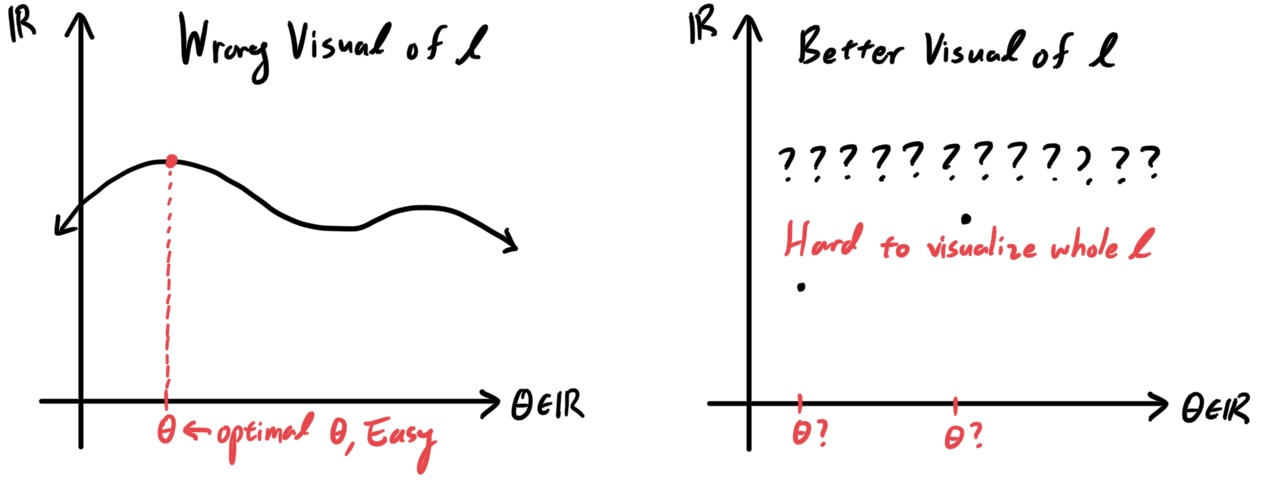
\includegraphics[width=0.6\textwidth]{img/visual_of_l.jpg}
    \caption{} 
    \label{fig:visual_of_l}
  \end{figure}

  Rather, all we can do is hope to take whatever easier-to-visualize, lower-bound functions and maximize them as much as we can in hopes of converging onto $l$. Let us walk through the first two iterations of the EM algorithm. We first initialize $\theta$ to, say $\theta_0$. This immediately induces the lower-bound ELBO-sum function $\sum_{i} \text{ELBO} (x^{(i)};\, p_Z^{*i}, \theta)$, which takes in multinomial density functions $p_Z^{*i} = p_1, p_2, \ldots$ and outputs different functions of $\theta$ that are valid lower bounds. Two of these possible lower-bound functions are shown (in green) for when we input some arbitrary density $p_1, p_2$. However, there exists a density $p_Z^{(i)}$ that produces not only the maximum possible lower-bound (called max ELBO, shown in red) but is equal to $l(\theta)$ for that density input $p_Z^{(i)}$. We maximize this function with respect to $\theta$ to get $\theta_1$ as our next assignment of $\theta$. 

  \begin{figure}[H]
    \centering 
    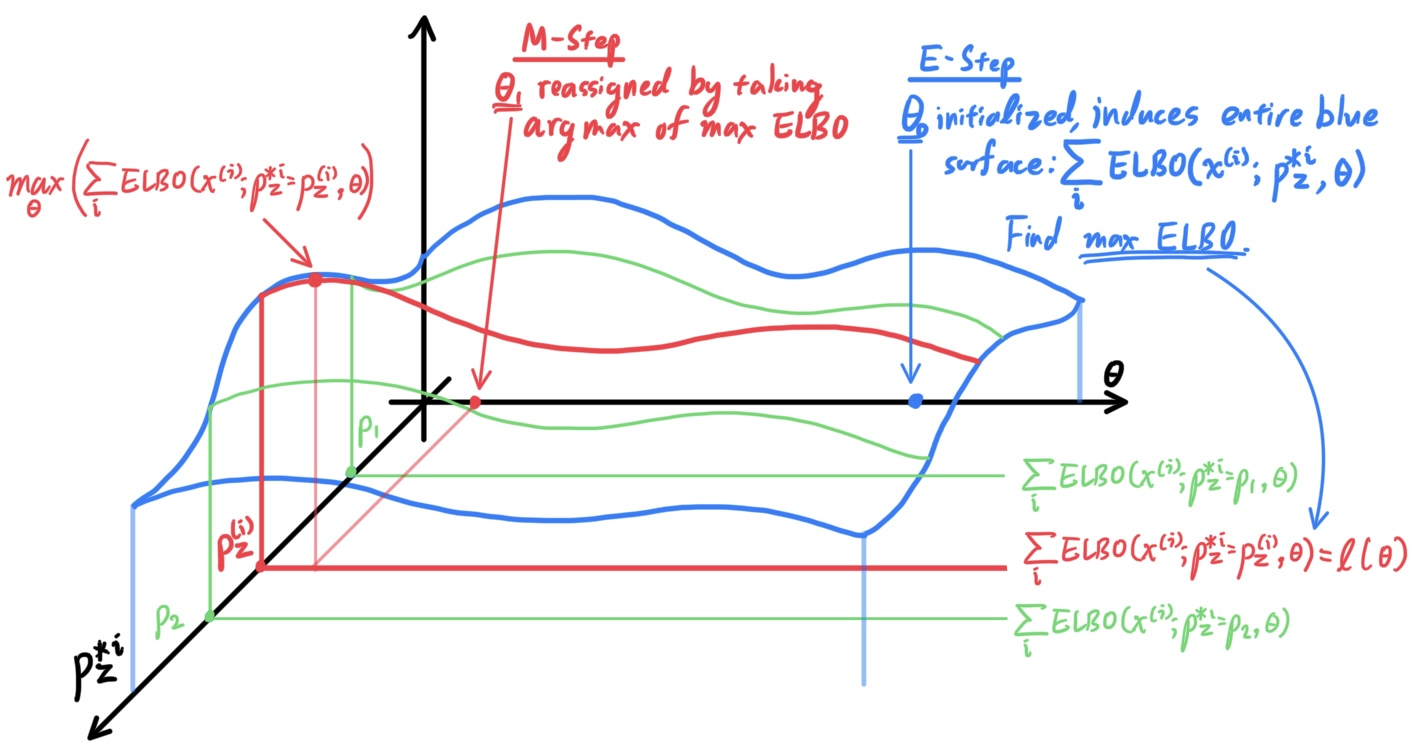
\includegraphics[width=0.7\textwidth]{img/EM_first_iteration.jpg}
    \caption{} 
    \label{fig:EM_first_iteration}
  \end{figure}

  The next step is identical. Now that we have a new value of $\theta = \theta_1$, this induces the lower-bound ELBO-sum function $\sum_{i} \text{ELBO} (x^{(i)};\, p_Z^{*i}, \theta)$ that also takes in multinomial densities $p_Z^{*i}$ and outputs different functions of $\theta$ that are valid lower-bounds. Two possible lower bounds are shown (in green), but the maximum lower-bound (in blue) is produced when we input density $p_Z^{(i)}$. Since this max ELBO function is equal to $\theta$ for this fixed density input $p_Z^{(i)}$, we maximize this function with respect to $\theta$ to get $\theta_2$ as our next assignment of $\theta$. 

  \begin{figure}[H]
    \centering 
    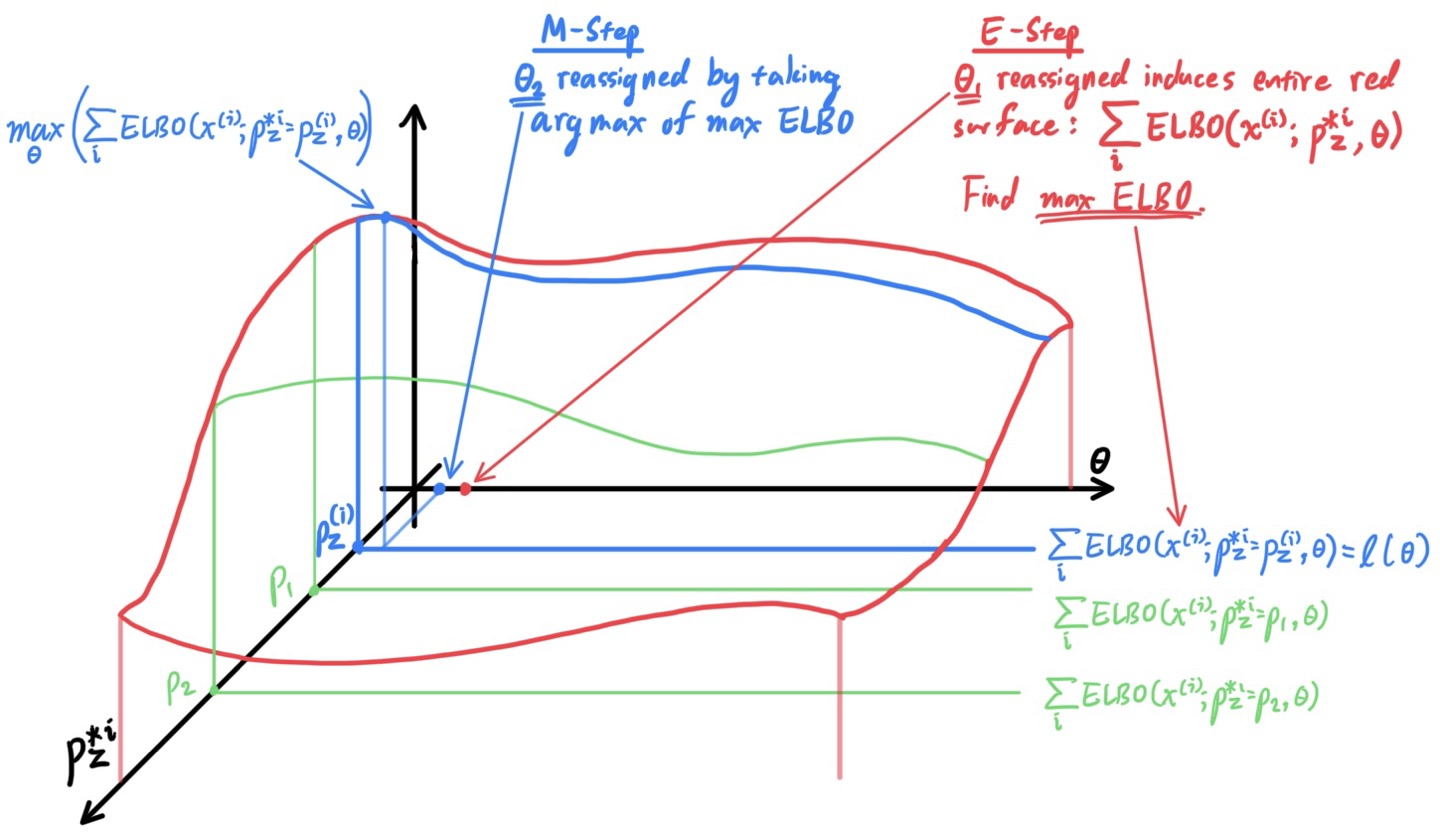
\includegraphics[width=0.7\textwidth]{img/EM_second_iteration.jpg}
    \caption{} 
    \label{fig:EM_second_iteration}
  \end{figure}

  \begin{definition}[EM Algorithm for General Estimation Problems]
    Given a training set $\{x^{(i)}\}_{i=1}^n \in \mathbb{R}^d$, let us assume that the random variable $X$ that these examples follow can be modeled by specifying a joint distribution of a multinomial and some arbitrary distributions. Let there be $k$ clusters, and let 
    \begin{itemize}
      \item $Z$ be the multinomial distribution representing which Gaussian cluster each example $x$ falls in, with density $p_Z (j)$ and represented by vector $\phi \in \mathbb{R}^k$ so that $\mathbb{P}(Z = j) = \phi_j$. Let the parameters of $\phi$ be encoded in $\theta$.
      \item The set of conditional distributions
        \[X\,|\,Z = j \sim X_j \text{ for } j = 1, 2, \ldots, k\]
      are arbitrary distributions with some parameters, also all encoded in $\theta$.  
    \end{itemize}

    The EM algorithm is described as such: 
    \begin{enumerate}
      \item Initialize $\theta$.
      \item \textbf{(E Step)} Since $l(\theta)$ is bounded below for all $p_Z^{*1}, \ldots, p_Z^{*n}$ as 
        \[l(\theta) \equiv \sum_{i=1}^n \log p\big( x^{(i)}; \, \theta\big) \geq \sum_{i=1}^n \text{ELBO}\big( x^{(i)}; \, p_Z^{*i}, \theta\big)\]
      setting $p_Z^{*i} (j) = p_Z^{(i)} (j) = p_Z \big(j\,|\, x^{(i)}; \, \theta\big)$ for all $i = 1, \ldots, n$ would put $l$ into a new form for these specific fixed values of $p_Z^{*i}$. 
        \[l(\theta) = \sum_{i=1}^n \text{ELBO}\big(x^{(i)}; p_Z^{(i)}, \theta \big)\]
      \item \textbf{(M Step)} We maximize this equivalent form of $l(\theta)$ with respect to $\theta$ whilst fixing the choice of $p_Z^{(i)}$. That is, we set the value of $\theta$ as 
      \begin{align*}  
        \theta & = \text{arg}\; \max_\theta \sum_{i=1}^n \text{ELBO} \big( x^{(i)}; \, p_Z^{(i)}, \theta \big) \\
        & = \text{arg}\; \max_\theta \sum_{i=1}^n \sum_{j=1}^k p_Z^{(i)} (j)\; \log \bigg( \frac{p(x^{(i)}, Z = j; \, \theta)}{p_Z^{(i)} (j)} \bigg) \\
        & = \text{arg}\; \max_\theta \sum_{i=1}^n \sum_{j = 1}^k p_Z \big(j\,|\, x^{(i)}; \, \theta \big)\, \log \bigg( \frac{p(x^{(i)}, Z = j; \, \theta)}{p_Z \big(j\,|\, x^{(i)}; \, \theta \big)} \bigg)
      \end{align*}
      \item We have successfully updated $\theta$. Now, we repeat steps 2 and 3 until convergence. Step 2 can bring improvements because we have changed the $\theta$, which means that there is a new sum of ELBO functions of the $\theta$ that serves as a new lower bound.
    \end{enumerate}
  \end{definition}

\subsection{Gaussian Mixture Models}

  Given a training set ${\mathbf{x}^{(i)}}_{i=1}^n$ (without the $y$-labels and so in the unsupervised setting), there are some cases where it may seem like we can fit multiple Gaussian distributions in the input space $\mathcal{X}$. For example, the points below seem like they can be fitted well with 3 Gaussians.

  \begin{figure}[H]
    \centering
    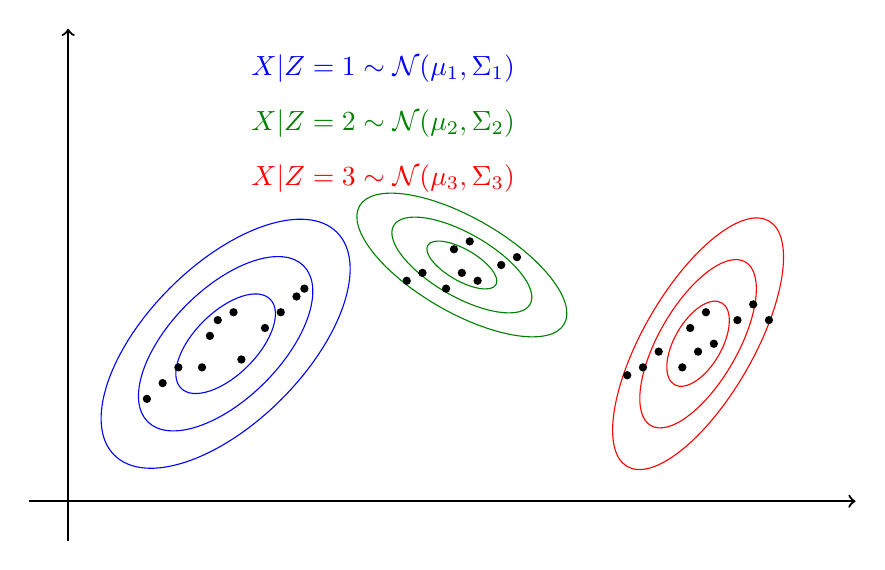
\begin{tikzpicture}
      % Draw axes
      \draw[black, ->, line width=0.8pt] (-0.5,0) -- (10,0);
      \draw[black, ->, line width=0.8pt] (0,-0.5) -- (0,6);
      
      % Equations at top
      \node[blue] at (4,5.5) {$X|Z=1 \sim \mathcal{N}(\mu_1, \Sigma_1)$};
      \node[green!50!black] at (4,4.8) {$X|Z=2 \sim \mathcal{N}(\mu_2, \Sigma_2)$};
      \node[red] at (4,4.1) {$X|Z=3 \sim \mathcal{N}(\mu_3, \Sigma_3)$};
      
      % First Gaussian (blue)
      \draw[blue, rotate around={45:(2,2)}] (2,2) ellipse (2 and 1);
      \draw[blue, rotate around={45:(2,2)}] (2,2) ellipse (1.4 and 0.7);
      \draw[blue, rotate around={45:(2,2)}] (2,2) ellipse (0.8 and 0.4);
      
      % Blue cluster points - more spread out
      \fill[black] (1.7,1.7) circle (1.5pt);
      \fill[black] (1.8,2.1) circle (1.5pt);
      \fill[black] (2.1,2.4) circle (1.5pt);
      \fill[black] (2.2,1.8) circle (1.5pt);
      \fill[black] (1.9,2.3) circle (1.5pt);
      \fill[black] (1.4,1.7) circle (1.5pt);
      \fill[black] (2.5,2.2) circle (1.5pt);
      \fill[black] (2.7,2.4) circle (1.5pt);
      \fill[black] (1.2,1.5) circle (1.5pt);
      \fill[black] (2.9,2.6) circle (1.5pt);
      \fill[black] (3.0,2.7) circle (1.5pt);
      \fill[black] (1.0,1.3) circle (1.5pt);
      
      % Second Gaussian (green)
      \draw[green!50!black, rotate around={-30:(5,3)}] (5,3) ellipse (1.5 and 0.6);
      \draw[green!50!black, rotate around={-30:(5,3)}] (5,3) ellipse (1 and 0.4);
      \draw[green!50!black, rotate around={-30:(5,3)}] (5,3) ellipse (0.5 and 0.2);
      
      % Green cluster points - more oval shaped
      \fill[black] (4.8,2.7) circle (1.5pt);
      \fill[black] (4.9,3.2) circle (1.5pt);
      \fill[black] (5.0,2.9) circle (1.5pt);
      \fill[black] (5.1,3.3) circle (1.5pt);
      \fill[black] (5.2,2.8) circle (1.5pt);
      \fill[black] (4.5,2.9) circle (1.5pt);
      \fill[black] (5.5,3.0) circle (1.5pt);
      \fill[black] (4.3,2.8) circle (1.5pt);
      \fill[black] (5.7,3.1) circle (1.5pt);
      
      % Third Gaussian (red)
      \draw[red, rotate around={60:(8,2)}] (8,2) ellipse (1.8 and 0.7);
      \draw[red, rotate around={60:(8,2)}] (8,2) ellipse (1.2 and 0.5);
      \draw[red, rotate around={60:(8,2)}] (8,2) ellipse (0.6 and 0.3);
      
      % Red cluster points - more spread out
      \fill[black] (7.8,1.7) circle (1.5pt);
      \fill[black] (7.9,2.2) circle (1.5pt);
      \fill[black] (8.0,1.9) circle (1.5pt);
      \fill[black] (8.1,2.4) circle (1.5pt);
      \fill[black] (8.2,2.0) circle (1.5pt);
      \fill[black] (7.5,1.9) circle (1.5pt);
      \fill[black] (8.5,2.3) circle (1.5pt);
      \fill[black] (7.3,1.7) circle (1.5pt);
      \fill[black] (8.7,2.5) circle (1.5pt);
      \fill[black] (8.9,2.3) circle (1.5pt);
      \fill[black] (7.1,1.6) circle (1.5pt);
    \end{tikzpicture}
    \caption{Example of data that can be fitted with 3 Gaussians}
  \end{figure}

  Therefore, we can construct a best-fit model as a composition of a multinomial distribution (to decide which one of the Gaussians $\mathbf{x}$ should follow) followed by a Gaussian. That is, to find the distribution of $\mathbf{x}$ and get the density function $p(\mathbf{x})$, we condition it on the random variable $Z$. More specifically, we let
  \begin{equation}
    Z \sim \text{Multinomial}(\boldsymbol{\phi}), \;\;\;\;\; \boldsymbol{\phi} = \begin{pmatrix} \phi_1 \ \phi_2 \ \ldots \ \phi_k \end{pmatrix} \text{ such that } \sum_{i=1}^k \phi_i = 1
  \end{equation}
  and define the conditional distributions as
  \begin{align*}
    \mathbf{X} \mid Z = 1 & \sim \mathcal{N}(\boldsymbol{\mu}_1, \boldsymbol{\Sigma}_1) \\
    \mathbf{X} \mid Z = 2 & \sim \mathcal{N}(\boldsymbol{\mu}_2, \boldsymbol{\Sigma}_2) \\
    \ldots & \sim \ldots \\
    \mathbf{X} \mid Z = j & \sim \mathcal{N}(\boldsymbol{\mu}_j, \boldsymbol{\Sigma}_j) \\
    \ldots & \sim \ldots \\
    \mathbf{X} \mid Z = k & \sim \mathcal{N}(\boldsymbol{\mu}_k, \boldsymbol{\Sigma}_k)
  \end{align*}
  Therefore, our model says that each $\mathbf{x}^{(i)}$ was generated by randomly choosing $z^{(i)}$ from ${1, \ldots, k}$ according to some multinomial, and then the $\mathbf{x}^{(i)}$ was drawn from one of the $k$ Gaussians depending on $z^{(i)}$. This model is called the \textbf{mixture of Gaussians model}. The parameters of our model are: 

  \begin{itemize}
    \item The vector $\boldsymbol{\phi} \in \mathbb{R}^k$ (which really has $k-1$ parameters) characterizing the multinomial distribution.
    \item The set of vectors $\boldsymbol{\mu}_1, \boldsymbol{\mu}_2, \ldots, \boldsymbol{\mu}_k$ representing the mean vectors of each multivariate Gaussian. For simplicity, we'll denote this set of vectors as $\bm{\mu}$.
    \item The set of symmetric, positive-definite matrices $\boldsymbol{\Sigma}_1, \boldsymbol{\Sigma}_2, \ldots, \boldsymbol{\Sigma}_k$ representing the covariance matrices of each multivariate Gaussian. For simplicity, we'll denote this set of matrices as $\bm{\Sigma}$.
  \end{itemize}

  We can write down the log-likelihood of the given data $\mathbf{x}^{(i)}$'s as a function of all the parameters above as:

  \begin{align*}
    l (\boldsymbol{\phi}, \bm{\mu}, \bm{\Sigma}) & = \sum_{i=1}^n \log, p\big( \mathbf{x}^{(i)} ;  \boldsymbol{\phi}, \bm{\mu}, \bm{\Sigma} \big) \\
    & = \sum_{i=1}^n \log \bigg( \sum_{j=1}^k  p\big( \mathbf{x}^{(i)} \mid z^{(i)} = j ; \bm{\mu}, \bm{\Sigma} \big) , p\big( z^{(i)} = j; \boldsymbol{\phi}\big) \bigg)
  \end{align*}

  This equation above tells us the (log-) likelihood of the data landing on the $\mathbf{x}^{(i)}$'s given that we have parameters $\boldsymbol{\phi}, \bm{\mu}, \bm{\Sigma}$. Note that since we only know that the \textit{final} value of the $i$th sample is $\mathbf{x}^{(i)}$ and not anything at all about which value $z^{(i)}$ the $i$th sample had, there is an extra unknown in this model. That is, we do not know which one of the $k$ Gaussians the $\mathbf{x}^{(i)}$ was generated from. These values $z^{(i)}$ are called the \textbf{hidden/latent variables}.

  If we did know the values of the hidden variables $z^{(i)}$ (i.e. if we knew which of the $k$ Gaussians each $\mathbf{x}^{(i)}$ was generated from), then our log likelihood function would be much more simple since now, our givens will be both $\mathbf{x}^{(i)}$ \textit{and} $z^{(i)}$. Therefore, we don't have to condition on the $z^{(i)}$ and can directly calculate the log of the probability of us having sample values $(z^{(1)}, \mathbf{x}^{(1)}), (z^{(2)}, \mathbf{x}^{(2)}), \ldots, (z^{(n)}, \mathbf{x}^{(n)})$.

  \begin{align*}
    l(\boldsymbol{\phi}, \bm{\mu}, \bm{\Sigma}) & = \sum_{i=1}^n \log , p\big( \mathbf{x}^{(i)}; \boldsymbol{\phi}, \bm{\mu} ,\bm{\Sigma}\big) \\
    & = \sum_{i=1}^n \log, p\big( \mathbf{x}^{(i)}, z^{(i)}; \boldsymbol{\phi}, \bm{\mu} ,\bm{\Sigma}\big) \\
    & = \sum_{i=1}^n \log, p\big( \mathbf{x}^{(i)} \mid z^{(i)}; \bm{\mu}, \bm{\Sigma}) \; p\big( z^{(i)}; \boldsymbol{\phi} \big)
  \end{align*}

  This model, with known $z^{(i)}$'s, is basically the GDA model, which is easy to calculate. That is, the maximum values of $\boldsymbol{\phi}, \bm{\mu}, \bm{\Sigma}$ are:

  \begin{align*}
    \phi_j & = \frac{1}{n} \sum_{i=1}^n \mathbbm{1}_{z^{(i)} = j} \\
    \boldsymbol{\mu}_j & = \frac{\sum_{i=1}^n \mathbbm{1}_{z^{(i)} = j} \mathbf{x}^{(i)}}{\sum_{i=1}^n \mathbbm{1}_{z^{(i)} = j}} \\
    \boldsymbol{\Sigma}_j & = \frac{1}{\sum_{i=1}^n \mathbbm{1}_{z^{(i)} = j}} \sum_{i=1}^n \mathbbm{1}_{z^{(i)}} \big( \mathbf{x}^{(i)} - \boldsymbol{\mu}_j \big),\big(\mathbf{x}^{(i)} - \boldsymbol{\mu}_j \big)^T
  \end{align*}

  for $j = 1, \ldots, d$. But since we do \textit{not} know the values of $z^{(i)}$, we first try to "guess" the values of the $z^{(i)}$'s and then update the parameters of our model assuming our guesses are correct. Let us clarify some notation:

  \begin{itemize}
    \item The distribution that we will iteratively reassign over and over again is $Z$, with density $p_Z (z)$ that maps $z \mapsto \phi_z$, where $\boldsymbol{\phi}$ is a vector that represents the density. The algorithm will initialize $p_Z$ and have it converge to the true multinomial density. Note that $Z$ in this context could represent the true multinomial distribution $Z$ or could represent the distributions iteratively produced by the algorithm that should converge onto the true $Z$ (usually the latter).

    \item The $k$ Gaussian distributions that we will iteratively reassign over and over again is $\mathcal{N}_1, \mathcal{N}_2, \ldots, \mathcal{N}k$, with densities $p_{\mathcal{N}1}(\mathbf{x}), \ldots, p_{\mathcal{N}k}(\mathbf{x})$ that maps $\mathbf{x} \mapsto p_{\mathcal{N}j}(\mathbf{x})$.

    \item The distribution of the entire random variable $\mathbf{X}$ will have density $p_X(\mathbf{x})$. Since we are iteratively reassigning the densities $p_Z$ and $p{\mathcal{N}_j}$, this joint distribution of $\mathbf{X}$ will also get modified.
  \end{itemize}

  \begin{definition}[EM Algorithm]
    The \textbf{Expectation-Maximization (EM) Algorithm} has the following steps:

    \begin{enumerate}
      \item We initialize our values of $\theta$, which can be chosen randomly or by \textbf{K-means initialization} (not explained here).
      \begin{itemize}
        \item We can randomly assign our values of $\mu_j$'s and the $\Sigma_j$'s in $\mathbb{R}^d$.
        \item We can randomly assign the density of our guess multinomial $p_Z(z)$, represented by vector
        \[\phi = \begin{pmatrix} \phi_1 \\ \vdots \\ \phi_k \end{pmatrix} \text{ with } \sum_{j=1}^k \phi_j = 1\]
        where $p_Z(z) \equiv \phi_z$ for $z = 1, \ldots, k$.
      \end{itemize}

      \item \textbf{(E Step)} Now that we have our prior guess of what $Z$ and its density function $p_Z$ is, we can calculate its posterior density function by taking one observed example $x^{(i)}$ and modifying $p_Z$ to $p_Z^{(i)}$. This superscript $(i)$ on the distribution $p_Z$ indicates that this is a posterior density created from observing $x^{(i)}$. (The motivation for this construction is explained more specifically in the next section involving Jensen's inequality.) Using Bayes' rule, we should calculate $n$ density functions
      \[p_Z^{(i)}(z) \equiv p_Z(z\,|\,x^{(i)}; \phi, \mathbf{\mu}, \mathbf{\Sigma}) \text{ for } i = 1, \ldots, n\]
      For easier notation, we let $\phi^{(i)}$ be the vector representation of the density $p_Z^{(i)}$. That is,
      \[\phi^{(i)} = \begin{pmatrix} \phi_1^{(i)} \\ \vdots \\ \phi_k^{(i)} \end{pmatrix} \text{ with } \sum_{j=1}^k \phi_j^{(i)} = 1\]
      where $p_Z^{(i)}(z) \equiv \phi^{(i)}_z$ for $z = 1, \ldots, k$ and $0$ otherwise. Then, we can calculate $\phi^{(i)}$ (and therefore $p_Z^{(i)}$) component-wise by calculating each $\phi_j^{(i)}$ (which is the probability of a point being in the $j$th cluster, given that we observe example $x^{(i)}$):
      \begin{align*}
          \phi_j^{(i)} &= p_Z^{(i)}\big(z = j;\, \phi, \mathbf{\mu}, \mathbf{\Sigma}\big) \\
          &= p_Z\big(z = j\,|\,x^{(i)};\,\phi, \mathbf{\mu}, \mathbf{\Sigma}\big) \\
          &= \frac{p_{\mathcal{N}_j}\big(x^{(i)}\,|\,z^{(i)} = j;\,\mathbf{\mu}, \mathbf{\Sigma}\big) \; p_Z\big(z^{(i)} = j;\,\phi\big)}{p_X\big(x^{(i)};\,\phi, \mathbf{\mu}, \mathbf{\Sigma}\big)} \\
          &= \frac{p_{\mathcal{N}_j}\big(x^{(i)}\,|\,z^{(i)} = j;\,\mathbf{\mu}, \mathbf{\Sigma}\big) \; p_Z\big(z^{(i)} = j;\,\phi\big)}{\sum_{l=1}^k p_{\mathcal{N}_j}\big(x^{(i)}\,|\,z^{(i)} = l;\,\mathbf{\mu}, \mathbf{\Sigma}\big)\; p_Z\big(z^{(i)} = l;\,\phi\big)}
      \end{align*}
      Note that we have everything we need to calculate the posterior probability distribution $p_Z^{(i)}(z)$ of a point being in any cluster.
      \begin{itemize}
          \item $p_{\mathcal{N}_j}(x^{(i)}\,|\,z^{(i)} = j)$ represents the conditional Gaussian density, which is completely defined because the parameters $\mu_j, \Sigma_j$ are already defined in initialization.
          \item $p_Z(z^{(i)} = j; \phi)$ is really just the probability $\phi_j$ that a given point is in the $j$th cluster, which we've also defined in initialization.
          \item $p_X(x^{(i)})$ represents the distribution of the entire random variable $X$ of the entire training set. Knowing the first two and taking the sum gives this density function $p_X$.
      \end{itemize}
      Therefore, we should end up with $n$ different $k$-vectors $\phi^{(1)}, \phi^{(2)}, \ldots, \phi^{(n)}$, each representing our best guess of what multinomial density $p_Z^{(i)}$ each $x^{(i)}$ had followed in order to be at the given points.


      \begin{figure}[H]
        \centering
        \begin{subfigure}[b]{0.48\textwidth}
          \centering
          \begin{tikzpicture}[scale=1.]
            \draw[->] (-0.5,0) -- (5,0);
            \draw[->] (0,-0.5) -- (0,3.5);
            
            % Points and labels
            \fill[red] (1,1) circle (3pt);
            \fill[red] (1.5,0.8) circle (3pt);
            \fill[red] (2,1.5) circle (3pt);
            \node[red] at (3,1.5) {$\phi_1=\frac{3}{6}$};
            
            \fill[blue] (3,2.5) circle (3pt);
            \fill[blue] (3.2,2) circle (3pt);
            \node[blue] at (4,2.5) {$\phi_2=\frac{2}{6}$};
            
            \fill[green!50!black] (4,1) circle (3pt);
            \node[green!50!black] at (4.5,1) {$\phi_3=\frac{1}{6}$};
          \end{tikzpicture}
          \caption{Hard label assignments.}
          \label{fig:hard-guesses}
        \end{subfigure}
        \hfill 
        \begin{subfigure}[b]{0.48\textwidth}
          \centering
          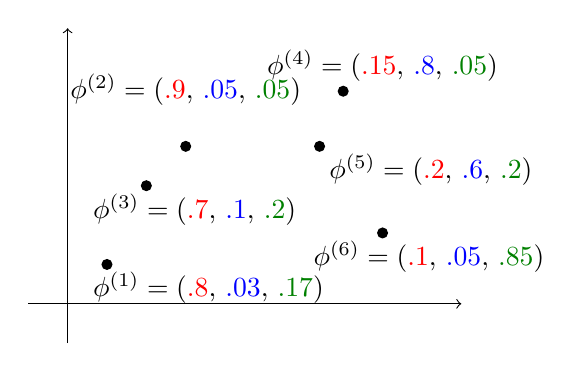
\begin{tikzpicture}[scale=1]
            \draw[->] (-0.5,0) -- (5,0);
            \draw[->] (0,-0.5) -- (0,3.5);
            
            % Points and colored vectors
            \fill (0.5,0.5) circle (2pt);
            \node[right] at (0.2,0.2) {$\phi^{(1)} = ($\textcolor{red}{.8}, \textcolor{blue}{.03}, \textcolor{green!50!black}{.17}$)$};
            
            \fill (1.5,2) circle (2pt);
            \node[above] at (1.5,2.4) {$\phi^{(2)} = ($\textcolor{red}{.9}, \textcolor{blue}{.05}, \textcolor{green!50!black}{.05}$)$};
            
            \fill (1,1.5) circle (2pt);
            \node[right] at (0.2,1.2) {$\phi^{(3)} = ($\textcolor{red}{.7}, \textcolor{blue}{.1}, \textcolor{green!50!black}{.2}$)$};
            
            \fill (3.5,2.7) circle (2pt);
            \node[above] at (4,2.7) {$\phi^{(4)} = ($\textcolor{red}{.15}, \textcolor{blue}{.8}, \textcolor{green!50!black}{.05}$)$};
            
            \fill (3.2,2) circle (2pt);
            \node[right] at (3.2,1.7) {$\phi^{(5)} = ($\textcolor{red}{.2}, \textcolor{blue}{.6}, \textcolor{green!50!black}{.2}$)$};
            
            \fill (4,0.9) circle (2pt);
            \node[right] at (3,0.6) {$\phi^{(6)} = ($\textcolor{red}{.1}, \textcolor{blue}{.05}, \textcolor{green!50!black}{.85}$)$};
          \end{tikzpicture}
          \caption{Soft probability assignments.}
          \label{fig:soft-guesses}
        \end{subfigure}
        \caption{Let us elaborate further on the intuition of this step. In the normal GDA with given values of $z^{(i)}$, we have $\phi_j = \frac{1}{n} \sum_{i=1}^n 1\{z^{(i)} = j\} = \frac{1}{n}\big(\text{Number of Samples in }j\text{th Gaussian}\big)$, which is a sum of "hard" guesses, meaning that each $x^{(i)}$ is undoubtedly in cluster $j$ or not, and so to find out our best guess for the true vector $\phi$, all we have to do is find out the proportion of all examples in each of the $k$ groups and we're done (without needing to iterate). However, in our EM model, we do not know the $z^{(i)}$'s, and so the best we can do is give the \textit{probability} $\phi^{(i)}_j$ that $x^{(i)}$ is in cluster $j$. So for each point $x^{(i)}$, the model has changed from it being undoubtedly in group $z^{(i)} = j$ to it having a probability of being in $\phi^{(i)}_j$ for $j = 1, \ldots, k$.}
        \label{fig:guesses-comparison}
      \end{figure}

      \item \textbf{(M Step)} With these $n$ separate posterior estimates of $Z$ for each observation $x^{(i)}$, we can simply average all of them and say that our best estimate of $\phi$ is
      \[\phi = \frac{1}{n} \sum_{i=1}^n \phi^{(i)}\]
      We can interpret the vectors $\phi^{(i)}$ as tuples where $\phi^{(i)}_j$ describes the expected "portion" of each sample $x^{(i)}$ to be in group $j$. So, we are adding up all the "portions" of the points that are expected to be in cluster $j$ to get $\phi_j = \sum_{i=1}^n \phi_j^{(i)}$.

      Now, given the $j$th Gaussian cluster, we would like to compute its mean $\mu_j$. Since each $x^{(i)}$ has probability $\phi^{(i)}_j$ of being in cluster $j$, we can weigh each of the $n$ points by $\phi^{(i)}_j$ (which determines how "relevant" $x^{(i)}$ is to cluster $j$) and average these (already weighted) points to get our "best-guess" of the mean $\mu_j$.
      \[\mu_j = \frac{\sum_{i=1}^n \phi^{(i)}_j x^{(i)}}{\sum_{i=1}^n \phi_j^{(i)}}\]

      \begin{figure}[H]
        \centering 
        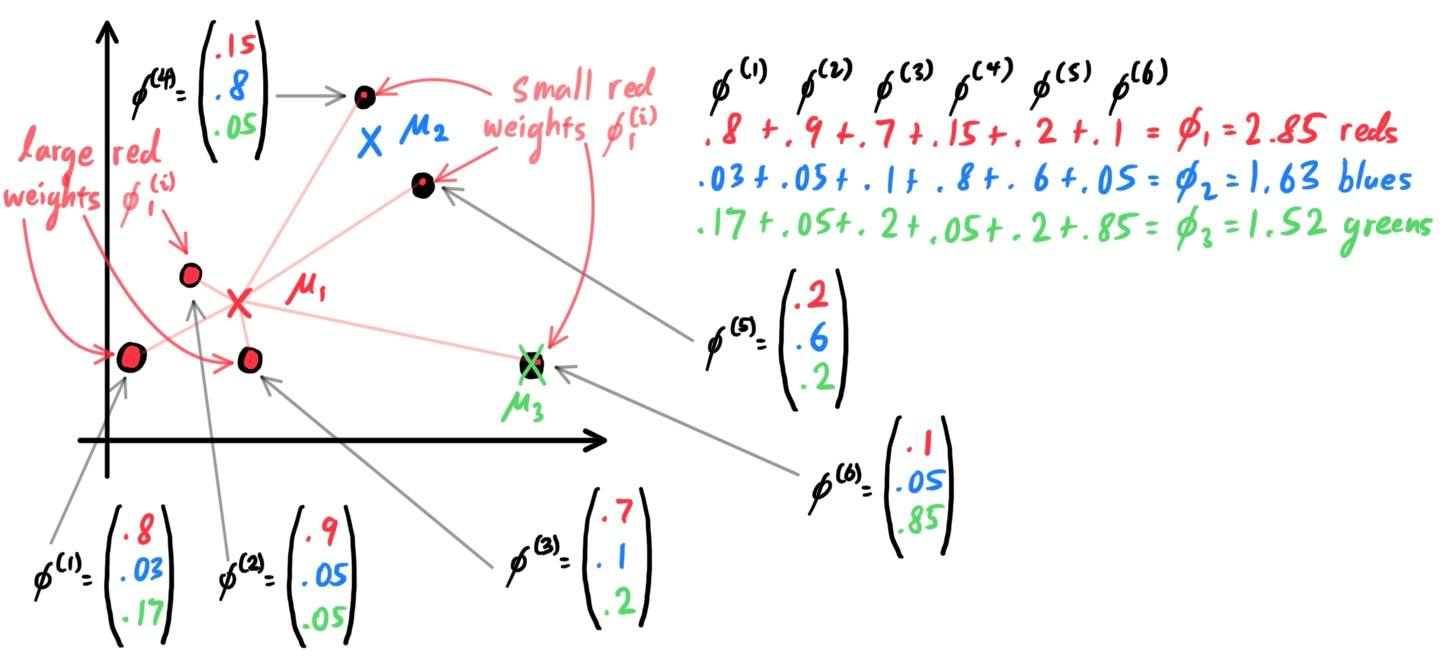
\includegraphics[scale=0.27]{img/weighted_means.jpg}
        \caption{} 
        \label{fig:weighted_means}
      \end{figure}

      With this logic of weighted points, we finally update the covariance matrices $\Sigma_j$ as below:
      \[\Sigma_j = \frac{1}{\sum_{i=1}^n \phi_j^{(i)}} \sum_{i=1}^n \phi^{(i)}_j \,\big(x^{(i)} - \mu_j\big)\big(x^{(i)} - \mu_j\big)^T\]

      \item Now, we have new values of $\phi, \mu_1, \ldots, \mu_k, \Sigma_1, \ldots, \Sigma_k$ that we can work with. With these new values, repeat steps 2 and 3 until convergence.
    \end{enumerate}
  \end{definition}

  In summary, this entire algorithm results from modifying the "hard" data of each point $x^{(i)}$ being undoubtedly in one cluster to a model containing points $x^{(i)}$ that have been "smeared" around different clusters, with a probability $\phi_j^{(i)}$ being in cluster $j$. 

  \begin{definition}[Mixture of Gaussians Algorithm: Summary]
    Given a training set $\{x^{(i)}\}_{i=1}^n \in \mathbb{R}^d$, let us assume that the random variable $X$ that these examples follow can be modeled by specifying a joint distribution of a multinomial and Gaussians. 
    That is, it follows a Gaussian mixture model (GMM) of $k$ Gaussian clusters. Let
    \begin{itemize}
      \item $Z$ be the multinomial distribution representing which Gaussian cluster each example $x$ falls in, with density represented by vector $\phi \in \mathbb{R}^k$ so that $\mathbb{P}(Z = j) \equiv \phi_j$.
      \item The set of conditional distributions 
        \[X\,|\,Z = j \sim \mathcal{N}(\mu_j, \Sigma_j) \text{ for } j = 1, 2, \ldots, k\]
      are multivariate Gaussian, with mean vectors $\mu_1, \ldots, \mu_k$ and covariance matrices $\Sigma_1, \ldots, \Sigma_k$. 
    \end{itemize}
    Let all the parameters be denoted as $\theta$. Then, the EM algorithm is as such: 
    \begin{enumerate}
      \item Initialize the multinomial vector $\phi$, the $\mu_j$'s, and the $\Sigma_j$'s.
      \item \textbf{(E Step)} Calculate the $n$ vectors
        \[\phi^{(i)} = \begin{pmatrix} \phi_1^{(i)} \\ \vdots \\ \phi_k^{(i)} \end{pmatrix} \text{ for all } i = 1, \ldots, n\]
      that represent the posterior distribution of $Z$ given observed $x^{(i)}$ by computing 
        \begin{align*} 
          \phi_j^{(i)} & = p_Z^{(i)} \big(z = j;\, \phi, \mathbf{\mu}, \mathbf{\Sigma} \big) \\
          & = p_Z \big(z = j\,|\, x^{(i)}; \, \phi, \mathbf{\mu}, \mathbf{\Sigma} \big) \\
          & = \frac{p_{\mathcal{N}_j} \big(x^{(i)}\,|\,z^{(i)} = j; \, \mathbf{\mu}, \mathbf{\Sigma}\big) \; p_Z \big(z^{(i)} = j;\, \phi \big)}{p_X \big(x^{(i)};\, \phi, \mathbf{\mu}, \mathbf{\Sigma}\big)} \\
          & = \frac{p_{\mathcal{N}_j} \big(x^{(i)}\,|\,z^{(i)} = j; \, \mathbf{\mu}, \mathbf{\Sigma}\big) \; p_Z \big(z^{(i)} = j;\, \phi \big)}{\sum_{l=1}^k p_{\mathcal{N}_j} \big( x^{(i)}\,|\, z^{(i)} = l;\, \mathbf{\mu}, \mathbf{\Sigma} \big)\; p_Z \big(z^{(i)} = l; \,\phi\big)}
        \end{align*}
      \item \textbf{(M Step)} Reassign the value of $\theta$ as 
        \begin{align*} 
          \phi & = \frac{1}{n} \sum_{i=1}^n \phi^{(i)} \\
          \mu_j & = \frac{\sum_{i=1}^n \phi_j^{(i)} x^{(i)}}{\sum_{i=1}^n w_j^{(i)}} \text{ for } j = 1, \ldots, n \\
          \Sigma_j & = \frac{1}{\sum_{i=1}^n \phi_j^{(i)}} \sum_{i=1}^n \phi^{(i)}_j \, \big(x^{(i)} - \mu_j \big) \big(x^{(i)} - \mu_j\big)^T \text{ for } j = 1, \ldots, n 
        \end{align*}
      \item Repeat steps 2 and 3 until convergence.
    \end{enumerate}
  \end{definition}

\subsection{Nonlinear ICA} 
